\documentclass{standalone}
\usepackage{tikz}
\usetikzlibrary{patterns, positioning}

\begin{document}
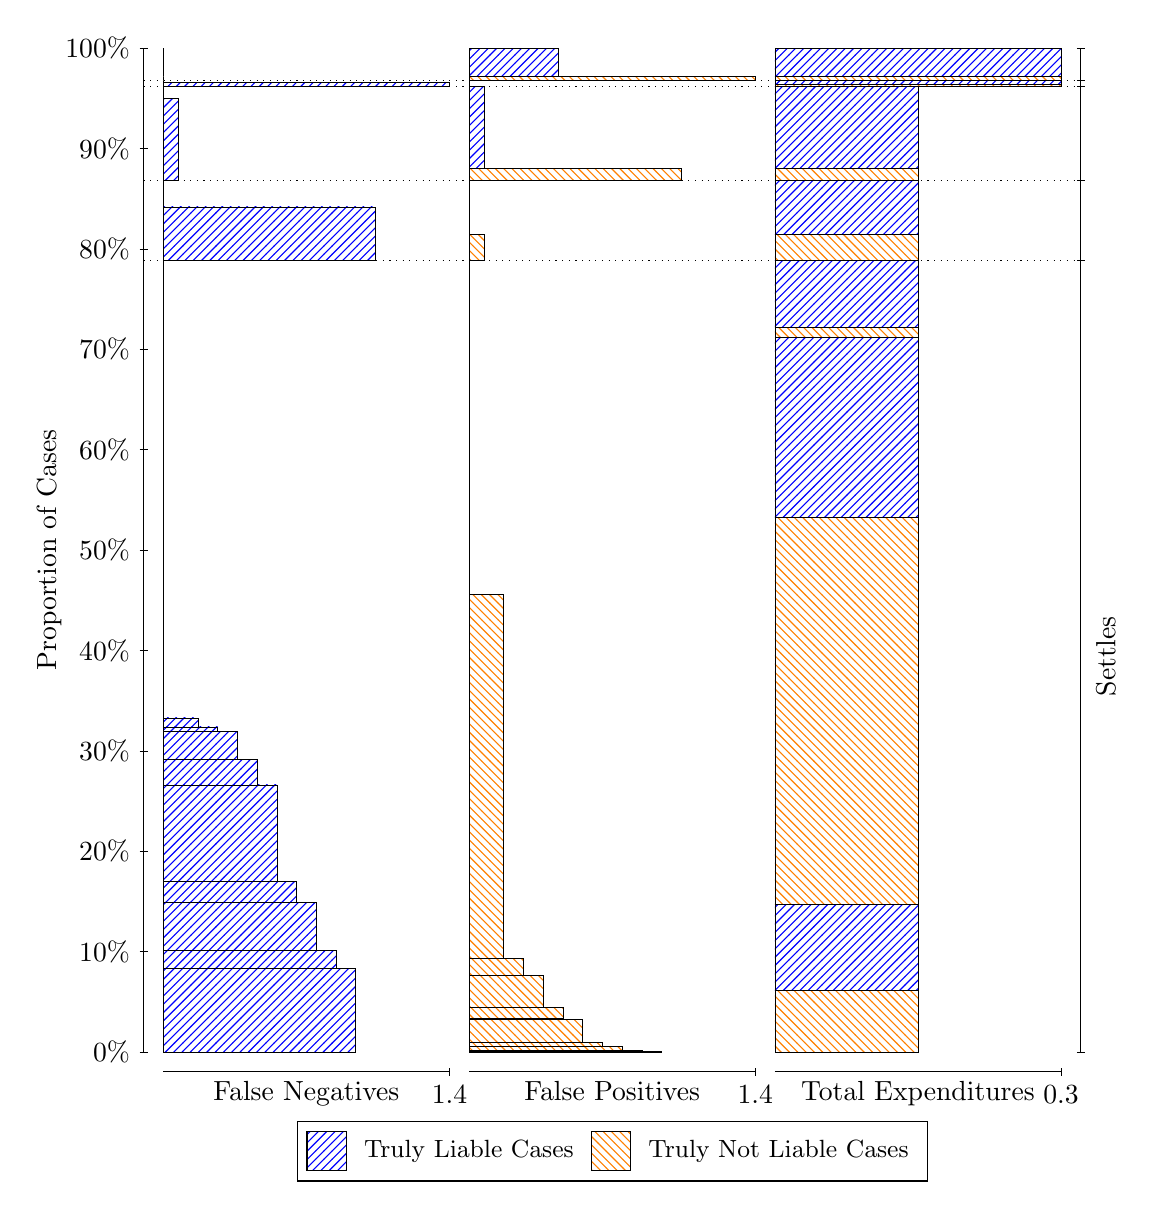
\begin{tikzpicture}
\draw[black, very thin] (1.5,1.75) -- (1.5,14.5);
\node[rotate=90, anchor=center] at (0.3, 8.125) {Proportion of Cases};
\draw[black, very thin] (1.45,1.75) -- (1.55,1.75);
\node[anchor=east] at (1.45, 1.75) {0\%};
\draw[black, very thin] (1.45,3.025) -- (1.55,3.025);
\node[anchor=east] at (1.45, 3.025) {10\%};
\draw[black, very thin] (1.45,4.3) -- (1.55,4.3);
\node[anchor=east] at (1.45, 4.3) {20\%};
\draw[black, very thin] (1.45,5.575) -- (1.55,5.575);
\node[anchor=east] at (1.45, 5.575) {30\%};
\draw[black, very thin] (1.45,6.85) -- (1.55,6.85);
\node[anchor=east] at (1.45, 6.85) {40\%};
\draw[black, very thin] (1.45,8.125) -- (1.55,8.125);
\node[anchor=east] at (1.45, 8.125) {50\%};
\draw[black, very thin] (1.45,9.4) -- (1.55,9.4);
\node[anchor=east] at (1.45, 9.4) {60\%};
\draw[black, very thin] (1.45,10.675) -- (1.55,10.675);
\node[anchor=east] at (1.45, 10.675) {70\%};
\draw[black, very thin] (1.45,11.95) -- (1.55,11.95);
\node[anchor=east] at (1.45, 11.95) {80\%};
\draw[black, very thin] (1.45,13.225) -- (1.55,13.225);
\node[anchor=east] at (1.45, 13.225) {90\%};
\draw[black, very thin] (1.45,14.5) -- (1.55,14.5);
\node[anchor=east] at (1.45, 14.5) {100\%};

\draw[black, very thin] (13.4,1.75) -- (13.4,14.5);
\draw[black, very thin] (13.35,1.75) -- (13.45,1.75);
\node[anchor=west] at (13.35, 1.75) {};
\draw[black, very thin] (13.35,11.8) -- (13.45,11.8);
\node[anchor=west] at (13.35, 11.8) {};
\draw[black, very thin] (13.35,12.82) -- (13.45,12.82);
\node[anchor=west] at (13.35, 12.82) {};
\draw[black, very thin] (13.35,14.015) -- (13.45,14.015);
\node[anchor=west] at (13.35, 14.015) {};
\draw[black, very thin] (13.35,14.089) -- (13.45,14.089);
\node[anchor=west] at (13.35, 14.089) {};
\draw[black, very thin] (13.35,14.5) -- (13.45,14.5);
\node[anchor=west] at (13.35, 14.5) {};

\draw[black, very thin, pattern color=blue, pattern=north east lines] (1.75,1.75) rectangle (4.1931,2.8164);
\draw[black, very thin, pattern color=blue, pattern=north east lines] (1.75,2.8164) rectangle (3.9425,3.0399);
\draw[black, very thin, pattern color=blue, pattern=north east lines] (1.75,3.0399) rectangle (3.692,3.6454);
\draw[black, very thin, pattern color=blue, pattern=north east lines] (1.75,3.6454) rectangle (3.4414,3.9172);
\draw[black, very thin, pattern color=blue, pattern=north east lines] (1.75,3.9172) rectangle (3.1908,5.1411);
\draw[black, very thin, pattern color=blue, pattern=north east lines] (1.75,5.1411) rectangle (2.9402,5.4618);
\draw[black, very thin, pattern color=blue, pattern=north east lines] (1.75,5.4618) rectangle (2.6897,5.8189);
\draw[black, very thin, pattern color=blue, pattern=north east lines] (1.75,5.8189) rectangle (2.4391,5.8777);
\draw[black, very thin, pattern color=blue, pattern=north east lines] (1.75,5.8777) rectangle (2.1885,5.9933);
\draw[black, very thin, pattern color=orange, pattern=north west lines] (1.75,5.9933) rectangle (1.75,11.8);
\draw[black, very thin, pattern color=blue, pattern=north east lines] (1.75,11.8) rectangle (4.4437,12.483);
\draw[black, very thin, pattern color=orange, pattern=north west lines] (1.75,12.483) rectangle (1.75,12.82);
\draw[black, very thin, pattern color=blue, pattern=north east lines] (1.75,12.82) rectangle (1.9379,13.859);
\draw[black, very thin, pattern color=orange, pattern=north west lines] (1.75,13.859) rectangle (1.75,14.015);
\draw[black, very thin, pattern color=blue, pattern=north east lines] (1.75,14.015) rectangle (5.3833,14.061);
\draw[black, very thin, pattern color=orange, pattern=north west lines] (1.75,14.061) rectangle (1.75,14.089);
\draw[black, very thin, pattern color=orange, pattern=north west lines] (1.75,14.089) rectangle (1.75,14.136);
\draw[black, very thin, pattern color=blue, pattern=north east lines] (1.75,14.136) rectangle (1.75,14.5);
\draw[black, very thin, pattern color=orange, pattern=north west lines] (5.6333,1.75) rectangle (8.0764,1.7606);
\draw[black, very thin, pattern color=orange, pattern=north west lines] (5.6333,1.7606) rectangle (7.8259,1.7682);
\draw[black, very thin, pattern color=orange, pattern=north west lines] (5.6333,1.7682) rectangle (7.5753,1.8207);
\draw[black, very thin, pattern color=orange, pattern=north west lines] (5.6333,1.8207) rectangle (7.3247,1.8723);
\draw[black, very thin, pattern color=orange, pattern=north west lines] (5.6333,1.8723) rectangle (7.0741,2.1606);
\draw[black, very thin, pattern color=orange, pattern=north west lines] (5.6333,2.1606) rectangle (6.8236,2.1763);
\draw[black, very thin, pattern color=orange, pattern=north west lines] (5.6333,2.1763) rectangle (6.8236,2.32);
\draw[black, very thin, pattern color=orange, pattern=north west lines] (5.6333,2.32) rectangle (6.573,2.7231);
\draw[black, very thin, pattern color=orange, pattern=north west lines] (5.6333,2.7231) rectangle (6.3224,2.938);
\draw[black, very thin, pattern color=orange, pattern=north west lines] (5.6333,2.938) rectangle (6.0718,7.5567);
\draw[black, very thin, pattern color=blue, pattern=north east lines] (5.6333,7.5567) rectangle (5.6333,11.8);
\draw[black, very thin, pattern color=orange, pattern=north west lines] (5.6333,11.8) rectangle (5.8213,12.137);
\draw[black, very thin, pattern color=blue, pattern=north east lines] (5.6333,12.137) rectangle (5.6333,12.82);
\draw[black, very thin, pattern color=orange, pattern=north west lines] (5.6333,12.82) rectangle (8.327,12.976);
\draw[black, very thin, pattern color=blue, pattern=north east lines] (5.6333,12.976) rectangle (5.8213,14.015);
\draw[black, very thin, pattern color=orange, pattern=north west lines] (5.6333,14.015) rectangle (5.6333,14.043);
\draw[black, very thin, pattern color=blue, pattern=north east lines] (5.6333,14.043) rectangle (5.6333,14.089);
\draw[black, very thin, pattern color=orange, pattern=north west lines] (5.6333,14.089) rectangle (9.2667,14.136);
\draw[black, very thin, pattern color=blue, pattern=north east lines] (5.6333,14.136) rectangle (6.7609,14.5);
\draw[black, very thin, pattern color=orange, pattern=north west lines] (9.5167,1.75) rectangle (11.333,2.5274);
\draw[black, very thin, pattern color=blue, pattern=north east lines] (9.5167,2.5274) rectangle (11.333,3.6282);
\draw[black, very thin, pattern color=orange, pattern=north west lines] (9.5167,3.6282) rectangle (11.333,8.5351);
\draw[black, very thin, pattern color=blue, pattern=north east lines] (9.5167,8.5351) rectangle (11.333,10.825);
\draw[black, very thin, pattern color=orange, pattern=north west lines] (9.5167,10.825) rectangle (11.333,10.948);
\draw[black, very thin, pattern color=blue, pattern=north east lines] (9.5167,10.948) rectangle (11.333,11.8);
\draw[black, very thin, pattern color=orange, pattern=north west lines] (9.5167,11.8) rectangle (11.333,12.137);
\draw[black, very thin, pattern color=blue, pattern=north east lines] (9.5167,12.137) rectangle (11.333,12.82);
\draw[black, very thin, pattern color=orange, pattern=north west lines] (9.5167,12.82) rectangle (11.333,12.976);
\draw[black, very thin, pattern color=blue, pattern=north east lines] (9.5167,12.976) rectangle (11.333,14.015);
\draw[black, very thin, pattern color=orange, pattern=north west lines] (9.5167,14.015) rectangle (13.15,14.043);
\draw[black, very thin, pattern color=blue, pattern=north east lines] (9.5167,14.043) rectangle (13.15,14.089);
\draw[black, very thin, pattern color=orange, pattern=north west lines] (9.5167,14.089) rectangle (13.15,14.136);
\draw[black, very thin, pattern color=blue, pattern=north east lines] (9.5167,14.136) rectangle (13.15,14.5);
\draw[black, dotted] (1.5,11.8) -- (13.4,11.8);
\draw[black, dotted] (1.5,12.82) -- (13.4,12.82);
\draw[black, dotted] (1.5,14.015) -- (13.4,14.015);
\draw[black, dotted] (1.5,14.089) -- (13.4,14.089);
\draw[black, very thin] (1.75,1.5) -- (5.3833,1.5);
\node[anchor=north] at (3.5667, 1.5) {False Negatives};
\draw[black, very thin] (5.3833,1.45) -- (5.3833,1.55);
\node[anchor=north] at (5.3833, 1.45) {1.4};

\draw[black, very thin] (5.6333,1.5) -- (9.2667,1.5);
\node[anchor=north] at (7.45, 1.5) {False Positives};
\draw[black, very thin] (9.2667,1.45) -- (9.2667,1.55);
\node[anchor=north] at (9.2667, 1.45) {1.4};

\draw[black, very thin] (9.5167,1.5) -- (13.15,1.5);
\node[anchor=north] at (11.333, 1.5) {Total Expenditures};
\draw[black, very thin] (13.15,1.45) -- (13.15,1.55);
\node[anchor=north] at (13.15, 1.45) {0.3};

\node[black, centered, rotate=90] at (13.72, 6.775) {Settles};





\draw (7.449999999999999,1.5) node[draw=none] (baseCoordinate) {};
\begin{scope}[align=center]
        \matrix[scale=0.5, draw=black, below=0.5cm of baseCoordinate, nodes={draw}, column sep=0.1cm]{
            \node[rectangle, draw, minimum width=0.5cm, minimum height=0.5cm, pattern=north east lines, pattern color=blue] {}; &
            \node[draw=none, font=\small] (B) {Truly Liable Cases}; &
            \node[rectangle, draw, minimum width=0.5cm, minimum height=0.5cm, pattern=north west lines, pattern color=orange] {}; &
            \node[draw=none, font=\small] (B) {Truly Not Liable Cases}; \\
            };
\end{scope}

\end{tikzpicture}
\end{document}